\subsection{Overview}
In order to design our application we need two main parts: one is the
The general architecture of our system has three tiers.
We have a mobile app running on mobile devices, smartphones or tablets with ios or Android.
then we have a server

the kind of architecture is distributed logic as explainde in the slides.


\subsection{Component view}

\begin{sidewaysfigure}
\centering
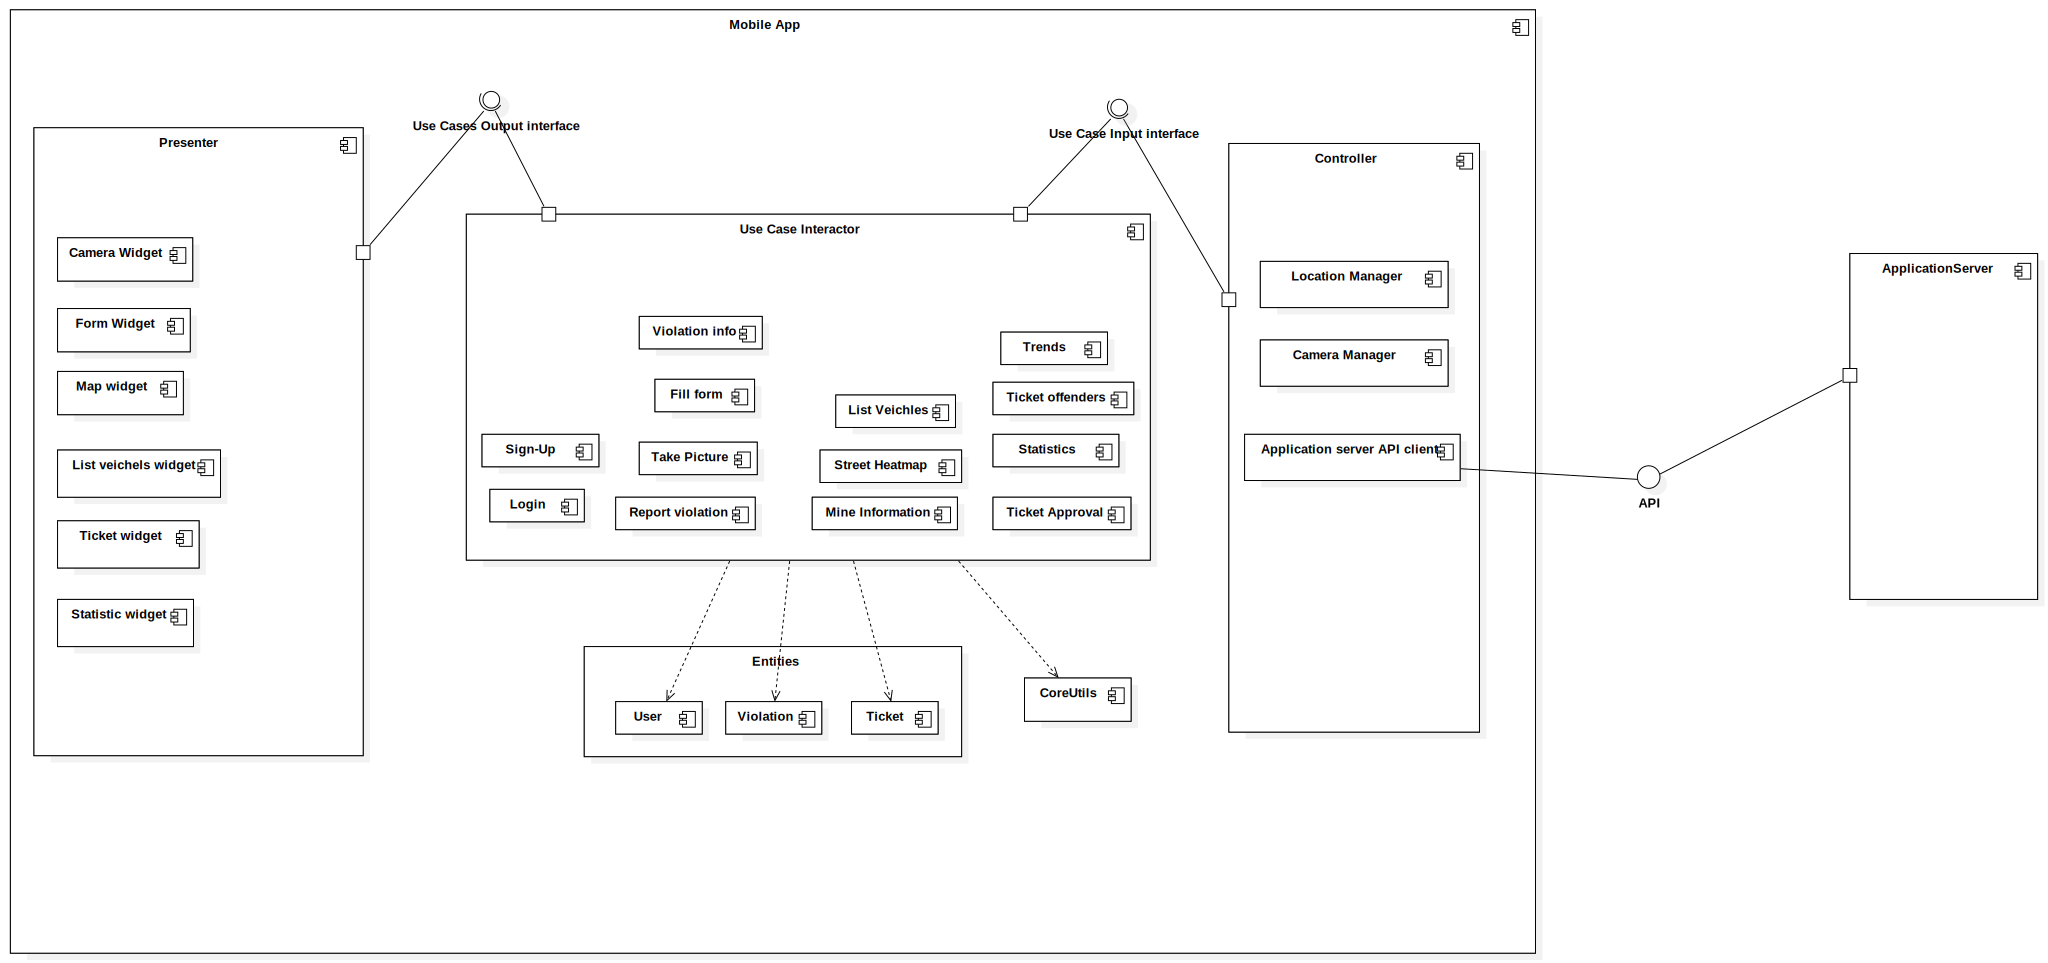
\includegraphics[width=\textwidth]{Images/ComponentDiagram1.png}
\caption{\label{fig:compdiag} Component diagram}
\end{sidewaysfigure}



\subsubsection{Mobile App}
The mobile application is the c

\subsection{Report Violation}
This component is responsible of showing the widget to take the camera.
\subsection{Form screen}
This component is needed after the picture has been taken to show the form where the user will select the kind of violation.

\subsection{Deployment view}

In Figure \ref{fig:deploy} is shown the Deployment diagram.

The deployment consist of three tiers. The first tier consist is \textbf{Mobile device} the user will use, which can be a smartphone or a tablet using as operating system either iOS or Android.
The exection environment is the built Flutter app.


The second tier is the \textbf{Application Server}. It is supposed to be a dedicated server running a linux distribution specific for server use. As an example of OS we choose Centos 7. Other distros can be used like Red Hat Enterprise Linux, Debian, OpenSUSE.
As execution enviorment we install Node.js which is an open-source JavaScript runtime environment that executes JavaScript code outside of a browser. Inside Node.js we use the web application framework Express.js which is designed for building web applications and APIs.


The third tier is the \textbf{DB Server}. It consists in another server where we run the DB system MongoDB. We choose to run the database in a separate server and not in the same as the ApplicationServer in order to increase scalability. MongoDB is a cross-platform document-oriented database program. Classified as a NoSQL database program, MongoDB uses JSON-like documents with schema.



\begin{figure}
\centering
\includegraphics[width=\textwidth]{Images/DeploymentDiagram1.png}
\caption{\label{fig:deploy} Deployment diagram}
\end{figure}



\subsection{Runtime view}

\subsection{Selected Architectural styles and patterns}



\subsection{Other design decisions}
